%Implementation

%General composition, functions, how to start a simulation, +-1 for up/down, wallArray contains wall agents, agentArray contains agents, simplifications, closest.m as discretization
\subsection{General considerations}
%ImplementationGeneral

\subsubsection{Introduction}
We had to build our implementation around several different desires:

\begin{itemize}
\item The code has to be expandable with additional features.
\item If there is a class model, it has to be simple because the project is not that big.
\item Constants should be easy to find and adjust.
\end{itemize}

\noi According to those points, the simulation code grew to be a mixture between classes and cascaded functions. At the top is a file defining all the global constants called  \textit{defineConstants.m}. This approach is maybe not very correct in terms of a good programming style, but it makes it very simple to adjust smaller details and to keep an overview over all the constants necessary to make the model work and to specify the field the agents walk in. It also provides an easy way to store and therefore document each run by simply saving the file containing all constants to a text file. All constants and variables are considered to be in SI-Units, if not mentioned otherwise. This means that all position specifications are given in meters, the velocity in meters per second and so on. Of course, this is only an approximation of reality, but it makes comparisons possible and easy.\\

\noi There are 3 classes implemented: \textit{simulation.m}, \textit{agent.m} and \textit{drawing.m}. A further description about these classes can be found in the table beneath or directly in the header of the class files. The rest of the code is split up into different logical functions.\\[12px]
\begin{tabular}{|l|p{7cm}|l|}
        \hline
        Class & Description & Parent \\ \hline
        simulation.m
		& This class offers all the functions for simulations. It can be executed  
		with different parameters depending on the users preferences.           
		& Matlab "handle" class \\ \hline
		agent.m    
		& This class is a container for all the agent data such as its radius, velocity and 
		position.   
		& Matlab "handle" class \\ \hline
		drawing.m
		& This class can draw a field containing agents.           
		& Matlab "handle" class \\  \hline
\end{tabular}\\[12px]

\noi The class diagram given in figure \ref{fig:classpackage} is a summary of the most important functions and properties in this project.\\

\begin{figure}[h!]
	\centering
		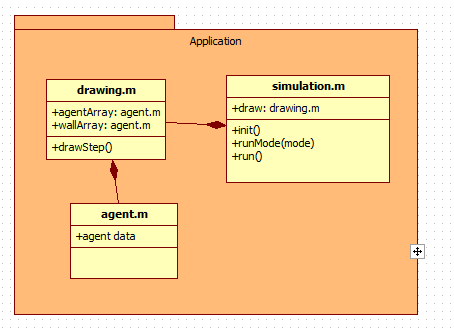
\includegraphics[width=0.70\textwidth]{pictures/classpackage}
	\caption{Class diagram of our model. From bottom to top we implemented a class \textit{agent.m}, \textit{drawing.m} and \textit{simulation.m}.}
	
\end{figure}

%simulation.m
\subsubsection{Important classes to run the simulation}
\noi The simulation class \textit{simulation.m} describes an object that wraps all the different possibilities of our simulation program. It's the starting point for a new simulation, runs this simulation and collects all the data requested from the agents and the simulated environment. The drawing class \textit{drawing.m} handles all graphical aspects of our simulation. The agent class \textit{agent.m} has a subchapter of its own because it fulfills a very different role than the two classes mentioned previously.\\
The main flow of a run cycle is described in the activity diagram given in figure \ref{fig:activityDiagram}.\\


\begin{figure}[h!]
	\centering
		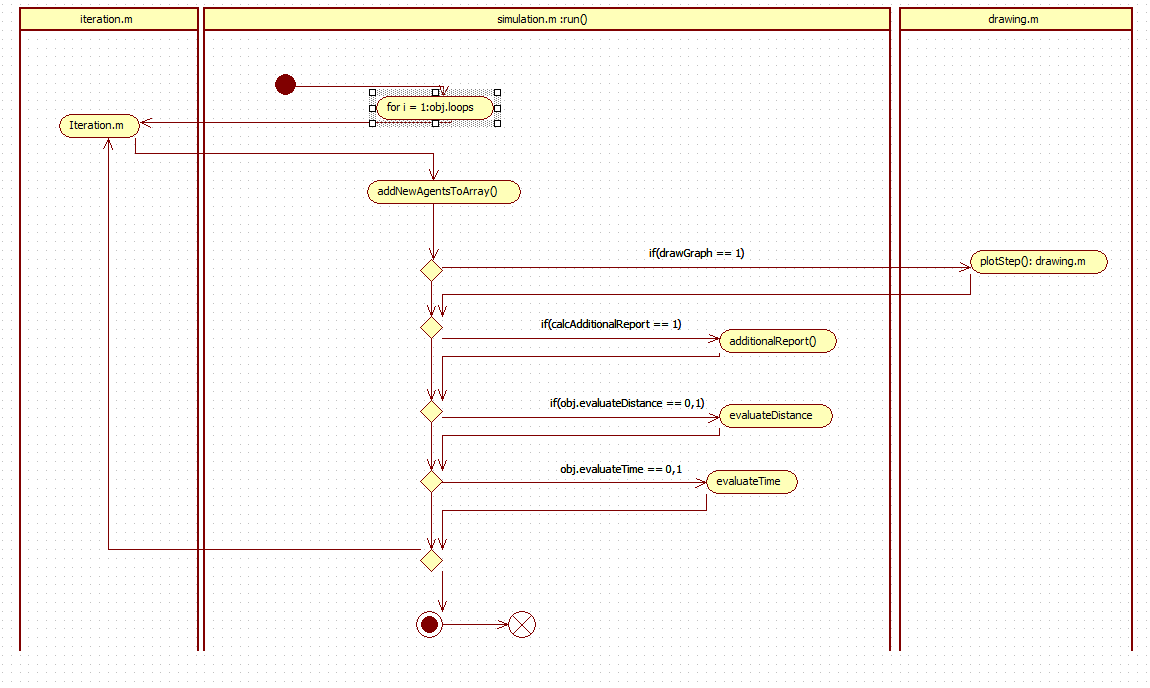
\includegraphics[width=0.70\textwidth]{pictures/activityDiagram}
	\caption{Activity diagram of our model.}
	\label{fig:activityDiagram}
\end{figure}

\noi Important properties of the simulation class \textit{simulation.m} are:
\begin{itemize}
\item \textsc{draw}: The \textit{drawing.m} implementation.
\item \textsc{result}: A matrix containing simulation results.
\item \textsc{additionalResult}: A matrix containing further simulation results.
\item \textsc{evaluateTime}: A vector used to evaluate the time an agent has spent in the simulation during its existence. %Noch beschreiben
\item \textsc{evaluateDistance}: A vector used to evaluate the distance an agent has covered in the simulation during its existence. %Noch beschreiben
\end{itemize}

\noi All methods of the simulation class are listed here:
\begin{itemize}
\item \textsc{simulation()}: Constructor, sets up the object.
\item \textsc{init()}: Initializes the existing object: Fills up arrays with empty objects, sets up vectors, etc.
\item \textsc{runMode()}: Pass console like parameters to this function to run a simulation and choose between various runmodes.
\item \textsc{additionalReport()}: Fills the additionalResult matrix with data.
\item \textsc{calcPossibleAgents()}: Calculates the maximum possible number of agents for the set area. 
\item \textsc{randPrefix()}: Randomly generates -1 or 1 to set the spawnpoint (top or bottom), if wanted to. It was replaced by spawning probabilities for top and bottom.
\item \textsc{initialSpawn()}: Fills up the agent array with new \textit{agent.m} objects. They have priority 0 which corresponds to non-existing agents.
\item \textsc{addNewAgentsToArray()}: Used to add new agents to the simulation while running.
\item \textsc{balanceProbability()}: Balances the probabilities to spawn agents, if wanted to. It was replaced by spawning probabilities for top and bottom with given constant probability.
\item \textsc{run()}: Main function to run a simulation after everything is set up and ready. This function should not be executed directly by the user. New simulations should be started with the \textsc{runMode()} function.
\end{itemize}

\noi See also the activity diagram (figure \ref{fig:activityDiagram}) for a better overview on how these method functions are used in the simulation.\\

%drawing.m
\noi The drawing class \textit{drawing.m} basically adapts simple Matlab drawing functions and converts them into useful functions for this project. As a result it's very easy to draw the new situation after a simulation step by simply calling the method \textsc{plotStep()}.

\subsubsection{Properties}
Important properties are:
\begin{itemize}
\item \textsc{particleDensity}: Resolution for wall \textit{agent.m} objects in $\frac{\y{agents}}{\y{meter}}$.
\item \textsc{width}: The field width.
\item \textsc{length}: The field length.
\item \textsc{wallArray}: All the agent.m objects for the wall.
\item \textsc{agentArray}: All the agent.m objects for the simulation.
\end{itemize}

\subsubsection{Methods}
All methods are listed here:
\begin{itemize}
\item \textsc{drawing()}: Constructor, sets up the object.
\item \textsc{createWall()}: Creates wall agents according to the settings.
\item \textsc{plotStep()}: Main function, plots all the agents on a field with the walls and the starting lines. 
\item \textsc{drawWallSquares}: Draws the walls on the side.
\item \textsc{circlePlot}: Draws circles for the agents.
\item \textsc{drawLine}: Draws a line with coordinates. Used for the direction indicators etc.
\end{itemize}
\noi How the field is created is the subject of subchapter \ref{drawField}.

\subsubsection{Simplifications}
Some simplifications and constraints on the model had to be introduced during the implementation to keep the whole simulation manageable. At first, we decided that the agents should walk either up or down and used the sign of an agent's velocity as an indication in which direction the agent goes. In the logic functions, a discretization had to be introduced for the numerical evaluations of functions. To inter-convert values between different vectors, the function \textit{closest.m} was used.\\
\noi As a consequence of the model used for the logic functions, the agents will only be able to look forwards. Because of the actual way \textit{logicFunction.m} was implemented (see subchapter \ref{logic}), they would not use the full $\pm 90^\circ$ in front and on the side of them, but almost. We thought this not to be too critical as the human visual field is also smaller than $180^\circ$, if one doesn't move the head.\\
\noi If one walks through the main station, it is visible that many people are not on their own. Groups of people tend to walk together as they want to chat. This can be seen very clearly in couples which try to walk side-by-side. To incorporate this in our model, we would have to introduce some kind of coupling between agents, for example that they would always be below a certain distance from each other. As we constructed our model from scratch, we thought it should be challenging enough to make it work with completely independent agents and decided to make every agents independent of all others.\\
\noi The hallway in the main station in Zurich is approximately 60 meters long. We shortened the way to 30 meters as we reckon that the same effects should be visible over that length. This saves some time for the simulations as the way until the agents from the opposite directions meet is considerable shortened. Also, it is of practical use as one can observe more details in a less stretched picture.

\subsection{How to run a simulation}
To start a simulation, simply change to the "/code" directory in your local matlab installation. Then type "run" into the command window. This will set up a new simulation environment. This environment can be accessed trough the "sim" variable.\\
The run script will ask for a "runmode" and whether you'd like to save the data. Supported runmodes are:\\[12px]
\begin{tabular}{|p{3cm}|p{10cm}|}
      \hline
      normal & normal mode with many wall agents\\ \hline
      fasttest & faster mode with less wall agents \\ 
      \hline
\end{tabular}\\[12px]
\noi Supported parameters are:\\[12px]
\begin{tabular}{|p{3cm}|p{10cm}|}
      \hline
      -nograph & simulation draws no graph, can be used if graphical output is not necessary.\\ \hline
      -report & additional report will be recorded\\ \hline
      -nodirections & removes the direction markers on top of the agents.\\
      \hline
\end{tabular}\\[12px]
\noi A string could be for example: "normal -nograph -report". For a more detailed example please view the header of the run.m file. \\
\noi If one wants to save the data, type "Y" when asked and type in the name of the location/filename where the data shall be stored to. As a default, they are saved into the sim folder. Then the \textit{defineConstants.m} file containing all the constants is saved as a .txt file with the runmode appended. After the simulation is finished, the workspace variables containing the "sim" variable are saved as a .mat file. The situation after the last iteration is drawn and saved as a .png file, also when the parameter -nograph was called. This allows a first visual check on how a run went.


\subsection{Agents}
%Agents

As the model is agent-based, we wanted to implement them as such. Therefore we created a class called \text{agent.m}. Every agent has the following properties which are critical for the simulation:
\begin{itemize}
	\item Radius of the agent called \textsc{radius}
	\item The x coordinate of its position called \textsc{cordX}
	\item The y coordinate of its position called \textsc{cordY}
	\item A maximal velocity called \textsc{maxSpeed}
	\item An actual velocity called \textsc{actSpeed}
	\item A priority called \textsc{priority}
\end{itemize}
\noi Two more properties were introduced later for the analysis of the model. They are called \textsc{distance} and \textsc{time} and are used to monitor the time and pathlength an agent needs for crossing the field. The property \textsc{angle} stores the angle an agent wants to walk. This was used to graphically show the way they want to walk to during the simulation.\\

\noi A circle is the mathematically easiest shape to consider, especially for collision detections which have to be done later all the time. In addition, we consider the circle to be a good approximation as one also needs some space to move as the legs cover some space in front and behind the body. Also, a circle is very practical as it only needs one parameter entirely for the shape which is the radius. Using this approach, every agent can have a different radius.\\

\noi The coordinates of the agent with respect to a cartesian grid centered at the lower left of the whole filed are vital for all calculations. They are also needed to define the circle representing the agent in the plane. After each iteration, they will be adjusted to the new situation.\\

\noi Every agent has a maximum velocity. The actual velocity of an agent gives its actual speed. If there is no obstacle, it will be the maximum velocity. In the initialization of an agent, the first actual velocity is set to be equal to the maximum velocity. As velocity is in principle a vectorial quantity, we used the sign of the maximum velocity to determine the way an agent walks which is always well-defined as we don't let agents walk backwards. By our own convention, a positive sign means to go upwards (increasing y coordinate) and a negative sign means to go downwards (decreasing y coordinate).\\

\noi Every agent has a priority and usually a random number between 0 and 1. It is used to determine the order in which the agents move through one iteration step. A high priority means that the agent will walk first. A high priority value can be attributed to an agent which will always try to push his way through.\\
The priority is also used to mark inactive agents. As all arrays are stored in an array of class agent, a priority of 0 denotes an empty position and will not be drawn are considered. Any new agent is placed at the first position in the array of agents with a priority of 0. If an agent reaches its goal, it can be deleted by setting the priority to zero. This is the only time the priority value is changed after the creation of an agent.\\

\noi The class agent was implemented using \textit{handle} in the class definition. This has the same effect as \textit{call by reference} in C++ as there is after the creation only one instance of the agent, specially in the case where it is passed down to functions. A change of the value inside the function will be effective also outside the function which saves the step of giving the whole array of agents back after every function call which changes the coordinates or the actual velocity.


%class < handle




%How is the field drawn? (0/0) is bottom left, explain shortening the field
\subsection{Drawing of the field}\label{drawField}
%Implementierung der Zeichnung von Mosi!!!
To draw the field, the matlab API is used in a very basic way. Matlab supports the drawing of different shapes like circles, squares and lines. They can be combined in a single plot to create more complex graphic objects. The field is repainted after every simulation step by different functions. There is a separate function for the wall painting and to paint the spawn-lines on both sides. The agents are painted in two steps. First it paints a round "rectangle" to create a cyclic shape and then, if the user desires, direction indicators on top of it. All the drawing functions are processed in a procedural manner. Every agent is handled individually.\\

The field is defined by its wall agents. They could be in any shape. For example, if one wants extend the field with an obstacle somewhere between the spawn lines it can be defined by adding wall-agents to the specific coordinates. The easiest way to do so is to modify the createWall() function (which currently creates wall-agents on the left and the right side to simulate a hallway). Keep in mind that the coordinate system's zero point is on the lower left side. All wall agents are currently invisible.\\

If one does extend the field with other obstacles or different shaped walls and if it is not possible to frame the new situation with a simple geometric structure, the wall agents have to be drawn again. This is currently disabled because it slows down the simulation speed, and because the straight walls can be easily substituted with a long small rectangle. Drawing wall-agents is very simple due to the fact that they are exactly the same object type like a normal, moving agent. One can combine the two arrays (wall-agents and the moving agents) and let it draw by the iteration loop.\\

Currently, walls are coloured black, agents moving from top to bottom are painted in blue and those from bottom to top are red. The agent's direction indicators are painted black. All the distances are in meters.

%Description of the logical functions
\subsection{Logical functions}\label{logic}
%LogicFunctions.tex

\subsubsection{General considerations}
The heart of the simulation is the function \textit{logicFunction.m}, which determines the path any agent will choose to get to the other side of the hallway. To be more precise, it determines only the next step an agent will take and not the whole path. It relies heavily on the two functions \textit{xValuesLogic.m} to deal with other agents and \textit{xWallLogic.m} to deal with agents representing the wall or static obstacles. At first, the functioning of \textit{xValuesLogic.m} will be explained and afterwards the functioning of \textit{xWallLogic}.\\

\subsubsection{How to get $\beta_\y{Links}$ and $\beta_\y{Rechts}$?}
\begin{figure}[h!]
	\centering
		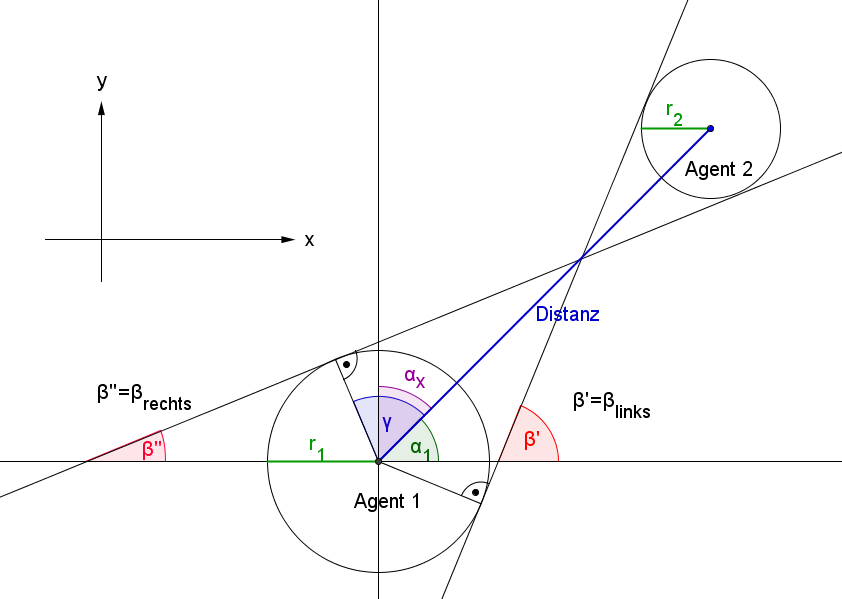
\includegraphics[width=0.80\textwidth]{pictures/beta.PNG}
	\caption{The graph shows the angles and variables used to get $\beta_\y{Links}$ and $\beta_\y{Rechts}$. $\alpha_X$ is the angle between the two agents with respect to the $y$-axis. This depiction was engineered to work also for agents walking the other way.}
	\label{fig:beta}
\end{figure}

\noi For our model, it is crucial to determine where an agent shouldn't go. The function \textit{getBeta.m} returns the angles which describe the interval of angles leading to a collision. A graphical depiction of the situation is given in figure \ref{fig:beta}. The equations (\ref{logik3}) to (\ref{logik5}) were used to get $\beta_\y{Links}$ and $\beta_\y{Rechts}$. They had to be converted into the angles given with respect to $\varphi$, $\beta_{\varphi,\y{ left}}$ and $\beta_{\varphi,\y{ right}}$ as shown in equations (\ref{logik6}) to (\ref{logik7}).
\begin{equation}\label{logik3}
	\gamma = arccos\brac{\frac{r_S}{d}},\ \alpha = arctan\brac{\frac{\Delta y}{\Delta x}}
\end{equation}
\begin{equation}\label{logik4}
	\beta_\y{Links} = \gamma + \alpha - \frac{\pi}{2}
\end{equation}
\begin{equation}\label{logik5}
	\beta_\y{Rechts} = \alpha + \frac{\pi}{2} - \gamma
\end{equation}
\begin{equation}\label{logik6}
  \beta_{\varphi,\y{ left}} = \frac{\pi}{2} - \beta_\y{Links} = \pi - (\gamma + \alpha)
\end{equation}
\begin{equation}\label{logik7}
  \beta_{\varphi,\y{ right}} = \frac{\pi}{2} - \beta_\y{Rechts} = \gamma - \alpha
\end{equation}
\noi This works between agents as well as between agents and the wall agents. Care was taken to engineer a calculation that allows for it to be used for agents walking in both directions.

\subsubsection{Calculation of the interaction with another dynamic agents}
\text{xValuesLogic.m} distinguishes three different cases.
\begin{itemize}
	\item For two crossing agents or if the agent in front of the agent in question is slower, we used equation (\ref{logik1}) to get $x_\y{out}'$. It was also used for two not moving agents, setting $\Delta v$ equal to an arbitrary value given in \texttt{STANDOFF}. This was a quick way to resolve standoffs, although this would eventually turn out to be in its actual form an Achilles heel of the model.
	\begin{equation}\label{logik1}
		x_\y{out}' = \frac{1}{\dis (|x - \alpha_X|)^{\brac{\frac{-\Delta v}{a}}}} = (|x - \alpha_X|)^{\brac{\frac{\Delta v}{a}}},\ \Delta v < 0
	\end{equation}
	\noi All values which correspond to a collision course in $x_\y{out}'$ are set to zero. This also deals with the singularity of equation (\ref{logik1}) as it is set to zero. This is done using the $\beta$-angles shown before. Afterwards, $x_\y{out}'$ is normalized and modificated further using equation (\ref{logik2}).
	\begin{equation}\label{logik2}
		x_\y{out} = x_\y{out}' \cdot \frac{b}{max(x_\y{out}')} \cdot \brac{\frac{r_S}{d}}^c
	\end{equation}
	\noi The variables $a$ (called \texttt{SLOPEFACTOR}), $b$ (\texttt{HEIGHT}) and $c$ (\texttt{REPULSIONAGENT}) have to chosen in a way that the simulation runs smoothly. The term $\frac{b}{max(x_\y{out}')}$ normalized the function to a maximum value $b$ while the term $\brac{\frac{r_S}{d}}^c$ controls that the repulsive influence gets stronger, the closer the two agents get. $c$ is usually chosen to be larger than 1.\\
	For two agents walking the in the same direction, the function given in equation \ref{logik2} is additionally multiplied with the difference in speed $|\delta v|$ in a try to make them avoid standing agents more resolute as it that case $|\delta v|$ would be rather big.\\
	
	\noi If the $x_\y{out}$ given in equation (\ref{logik2}) would be returned, the agent in question would aim to miss the other agent exactly. We thought that this would be too close as in reality, one also leaves a bit of space if possible between each other. Therefore we introduced an offset given as \texttt{WALLANGLEOFFSET} which gives the angle additionally to the $\beta$ angles for which an agent should aim to. To account for this, $x_\y{out}$ is modified with an linear interpolation between the values at $\beta + $\texttt{WALLANGLEOFFSET} and $\beta$ (which was set to zero before).

	\item If the agent in front of the agent in question is faster, a gaussian curve was used with the mean $\alpha_X$ and standard deviation $rS/d$. It is then modified further with $\Delta v$ and \texttt{HEIGHT} to make it a weak influence.
	\item For two agents moving with the same speed, the influence is set to zero by returning a vector of zeros.
\end{itemize}


\subsubsection{Calculation of the interaction with a wall agents}
To avoid hitting the wall, we used a very simple approach. Every angle corresponding to a collision course is set to a negative value accoring to equation (\ref{logik8}).
\begin{equation}\label{logik8}
	x_\y{Out} = x \cdot \frac{a}{d - rS}
\end{equation}
\noi As before for agents, an offset is introduced so the agent in question doesn't just try to avoid the wall-agent but also to leave some buffer space. The offset is also given in \texttt{WALLANGLEOFFSET}, $a$ can be accessed with the constant variable \texttt{WALLFACTOR}. $a$ has to be set negative as otherwise the wall would have an attracting force. To set a good value for this factor $a$ is quite delicate because if it is too low, agents will be stuck in the wall while if it too high, they will never approach the wall even slightly. 

\pagebreak
\subsubsection{Calculating functions in $x$ and transforming them into a polar axis in $\varphi$}
\begin{figure}[h!]
	\centering
		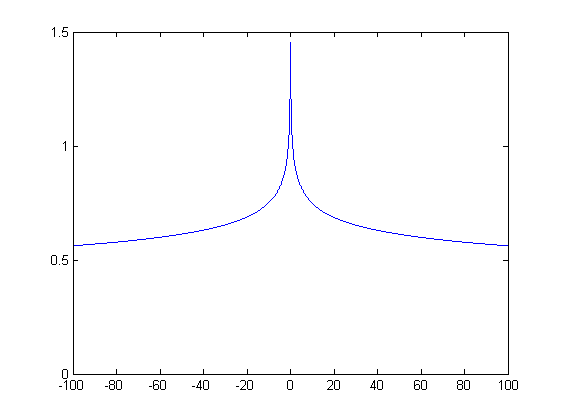
\includegraphics[width=0.40\textwidth]{pictures/Bsp2}
		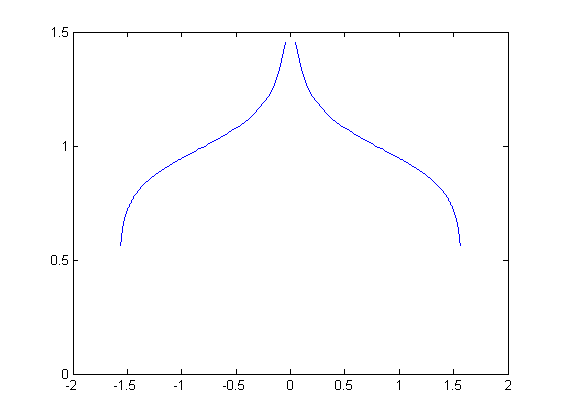
\includegraphics[width=0.40\textwidth]{pictures/Bsp2Angle}
	\caption{Graphical depiction of the function given in equation (\ref{logik1}). In the graphic on the left, the horizontal axis is given in $x$ while in the right graphic the horizontal axis is given in $\varphi$.}
	\label{fig:Bsp2}
\end{figure}

\noi As the functions given above are given in $x$ but the direction to go on is determined in polar values, it needs to be transformed into a $\varphi$ axis. This is done using a vector for $x$ ranging $\pm$ \texttt{XSCOPE} with a step of \texttt{XRES}. Applying the arcustangent on it yields the axis in angular values ($\varphi$). The transforming is done simply by using the $\varphi$ axis instead of the $x$ axis. This is shown in the two figures \ref{fig:Bsp2} and \ref{fig:Bsp2Out}. As those functions are only chosen to show the principle, they were not normalized in height according to the equations mentioned above.\\
\begin{figure}[h!]
	\centering
		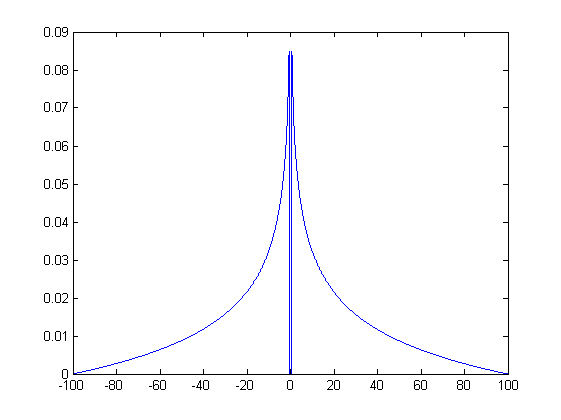
\includegraphics[width=0.40\textwidth]{pictures/Bsp2Out}
		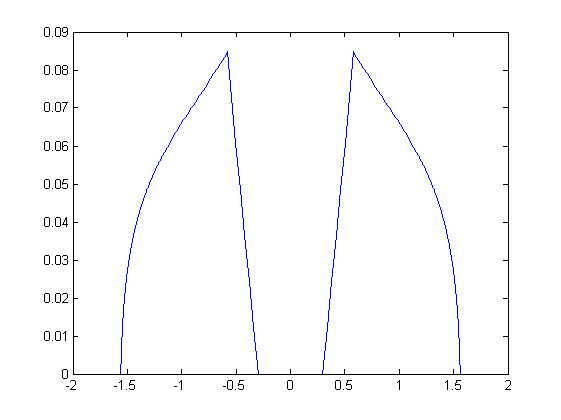
\includegraphics[width=0.40\textwidth]{pictures/Bsp2OutAngle}
	\caption{Graphical depiction of the return values of the function \textit{xValuesLogic.m}. In the graphic on the left, the horizontal axis is given in $x$ while in the right graphic the horizontal axis is given in $\varphi$. $\alpha_X$ was set to 0 corresponding to an other agent directly ahead, $\beta$ was set to $\pm 0.3$ with an offset of $0.25$.}
	\label{fig:Bsp2Out}
\end{figure}

In figure \ref{fig:Bsp2}, the function (\ref{logik1}) is shown graphically in the $x$ as well as $\varphi$ axis. Figure \ref{fig:Bsp2Out} shows the $x_\y{out}$ the function \textit{xValuesLogic.m} returns.



\subsubsection{Graphical example}
This subchapter shall give a visual example of how the logic functions work. Let's consider the situation given in figure \ref{fig:Bsp1}.
\begin{figure}[h!]
	\centering
		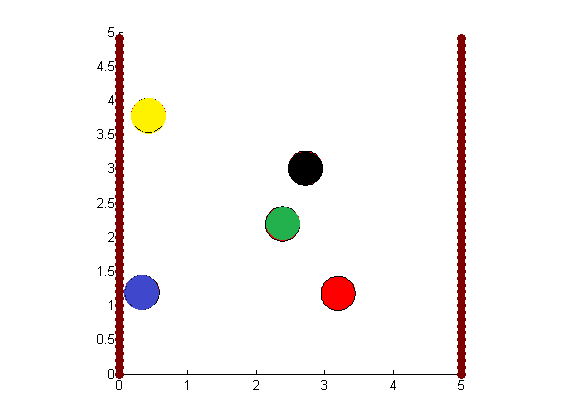
\includegraphics[width=0.45\textwidth]{pictures/Bsp1}
	\caption{Exemplary case used to demonstrate the working principle of the logic functions.}
	\label{fig:Bsp1}
\end{figure}

\noi The blue agent moving up in figure \ref{fig:Bsp1} only sees the influence of the wall. What the blue agent "sees" is given in figure \ref{fig:Bsp1LinksUnten}. The influence of the wall causes the overall function to decrease for all $\varphi$ corresponding to a collision course. The offset causes the overall function to have its maximum $\alpha$ at a positive $\varphi$. This causes the agent to walk in the direction of $\alpha$.\\
\begin{figure}[h!]
	\centering
		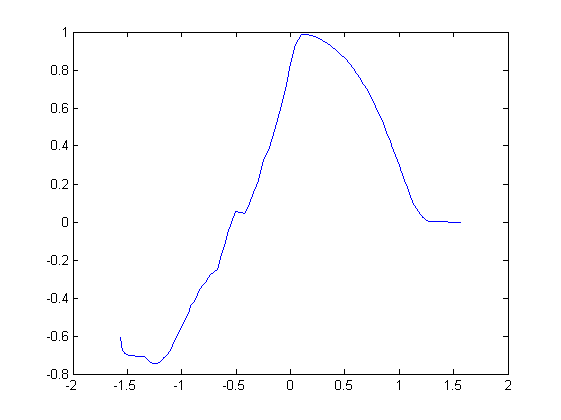
\includegraphics[width=0.4\textwidth]{pictures/Bsp1LinksUnten}
	\caption{Output of all logic functions combined for the blue agent in figure \ref{fig:Bsp1}. Visible is the effect of wall agents on the blue agent as negative values on the left side.}
	\label{fig:Bsp1LinksUnten}
\end{figure}

\noi The green agent moving up sees only the influence of the black agent who is moving down. The effect of that it given in figure \ref{fig:Bsp1Mitte}. The underlying gaussian function can be seen as well as the addition of a modified version of figure \ref{fig:Bsp2Out}, left. The agent will move slightly to the left to avoid hitting the black agent.\\
\begin{figure}[h!]
	\centering
		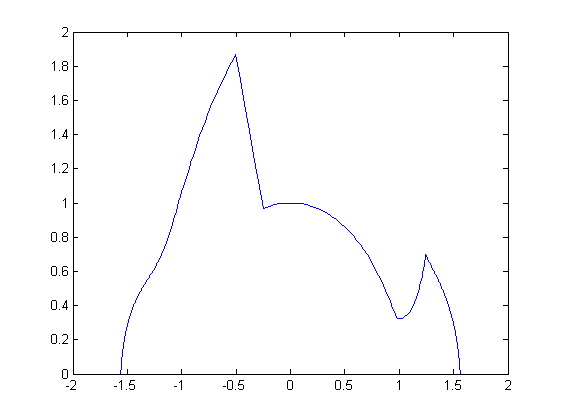
\includegraphics[width=0.40\textwidth]{pictures/Bsp1Mitte}
	\caption{Output of all logic functions combined for the green agent in figure \ref{fig:Bsp1}. Visible is the effect of the oncoming black agent as a superposition on the underlying gaussian curve.}
	\label{fig:Bsp1Mitte}
\end{figure}

\noi The black agent moving down sees the oncoming green and red agent going up. The effect of them is given in figure \ref{fig:Bsp1ObenRechts}. The superposition of two functions onto the underlying gaussion can be seen by the discontinities. The effect of the green agent is stronger as it is nearer to the black agent than the red agent which causes the black agent to go left (looking top-down) in order to avoid hitting the green agent. This shows the dependency of the strength of an agent of the distance.
\begin{figure}[h!]
	\centering
		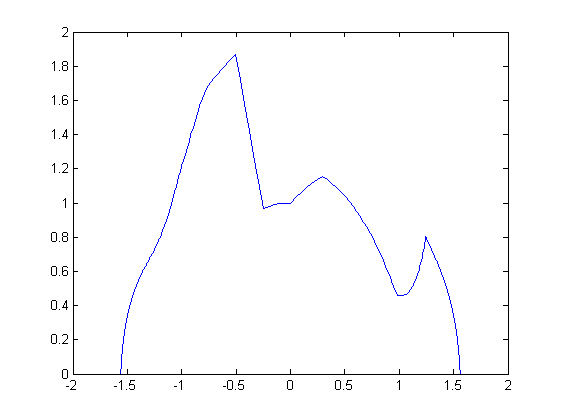
\includegraphics[width=0.40\textwidth]{pictures/Bsp1ObenRechts}
	\caption{Output of all logic functions combined for the black agent in figure \ref{fig:Bsp1}. Visible is the effect of the oncoming green and red agents as superpositions on the underlying gaussian curve. The black agent will move left (from his point of view) to avoid hitting the closer green agent.}
	\label{fig:Bsp1ObenRechts}
\end{figure}


%description of iteration function and collision detection, also spawning agents
\subsection{Iteration}
%Iteration

\subsubsection{General considerations}
One iteration step is carried out using the function \textit{Iteration.m}. For it to work properly, the array of all agents and all wall agents has to passed to it. All other inputs as well as all output variables are introduced for evalutation of the model and are per se not necessary for the iteration. It deals with three main tasks, the propagation of the simulation in time, the collision detection and the destruction of an agent after reaching its goal.\\
The spawning of new agents is treated in the function \textit{Spawn.m}. Both functions are called from the \textit{simulation.m} which controlls the simulation and stores all the data.

\subsubsection{Iteration step and collision detection}
This function takes four input array, although only two are critical for the success of the iteration. Those two are the arrays for all dynamic and static agents (equals wall agents). The output consists of the number of agents which disapeared during the iteration step, the distance covered by the disapeared agents as well as the time the disapeared agents had spent in the simulations.\\
At first, an index array is calculated with the indices of the dynamic agents in the given array of agents sorted according to their priority. This is done using the functions \textit{getPriorityArray.m} and \textit{getSortedPriorityArray.m}. Then a loop over the index array is carried out.\\
For every agent, the desired direction is calculated using the function \textit{logicFunction.m} explained above. Using the angle obtained by the call of \textit{logicFunction.m} und the speed given as the agent property, the new $x$- and $y$-coordiantes-to-be are determined. The path to it is then split in several substeps with the number of divisions given in the constant \texttt{PRECISIONCOLLISION}. In addition, the place where the agents stands is also included in case the agent cannot move at all.\\
For each of these positions, the distance to all other agents minus the radii is calculated yielding a distance matrix. This is done over all agents, dynamic as well as static. The last position for each other agent is left -1 as a sentinel. The distance matrix is then sorted using the matlab command \textit{sort} which leaves the most negative value for each column in the first row. The position of the first negative minimal distance indicates a collision. This position minus 1 will then be the distance the agent in question walks.\\

\noi In very rare cases, all positions in the first row of the sorted distance matrix are negative. This has the very nasty significance of an agent that could not even stand at its actual position. We reckon this has to do with some small numerical errors, as it only very rarely. To leave the agent at its actual position will now only result in a complete freze of two agents. It is certainly not a nice solution, but in these cases we simply deleted the faulty agent by setting its priority to 0 and reset its distance and time properties to enable the simulation to keep on running.

\subsubsection{Destruction of agents}
If an agent reaches his goal, the other side, it is automatically deleted inside \textit{Iteration.m}. This is simply done by setting the priority of the agent to 0. The attributes time and distance are read out before resetting and handed back to the calling function for later evaluation. After a deletion, the priority array giving all the indices of active agents is recalculated in order to avoid any influence of the deleted agent on other agents as the iteration step proceeds through the residual agents in the loop over all agents.

\subsubsection{Spawning new agents}
Spawning of one new agents is done by the function \textit{spawn.m}.



%Description of data readout
\subsection{Readout of informations of after a simulation}
\input{readout.tex}

%Description of the constant's definitions
\subsection{Defining all constants}
%constants.tex

\noi The file \textit{defineConstants.m} contains all the constants that are used somewhere in the simulation. They can be grouped into several categories which are listed below, only the most important and most frequently changed constants are listed explicitly.
\begin{itemize}
	\item The first section containing \texttt{XSCOPE} and \texttt{XRES} define the extent of the numerical approximations. An acceptable compromise between numerical resolution and runtime has to be chosen.
	\item In the second section, the model parameters can be set. They were explained in the subchapters about the logical functions and the spawning.
	\item The third section is used to define the field in which the agents whill walk.
	\item In the fourth and last section, general parameters concerning the simulation can be set. They include the time increment \texttt{DELTAT} and the number of loops \texttt{LOOPS} for the iteration process. The seed for the random number generator can be set with \texttt{SEED}.
\end{itemize}
\noi The seed for the random number generator is important to get random numbers but reproducible results.\\
Please note that early simulations may have a slightly different ordering of the constant variables in their logfiles.

\clearpage
